% TikZ diagram: distance zones for OBR distance rendering
% Radius normalized 0..1. 0..0.1 => in-head-localization, 0.1..1 => no change to spatialization
\documentclass[tikz,border=4mm]{standalone}
\usepackage{tikz}
\usepackage{xcolor}
\pagecolor{white}
\usetikzlibrary{arrows.meta,decorations.pathreplacing,calc}
\begin{document}
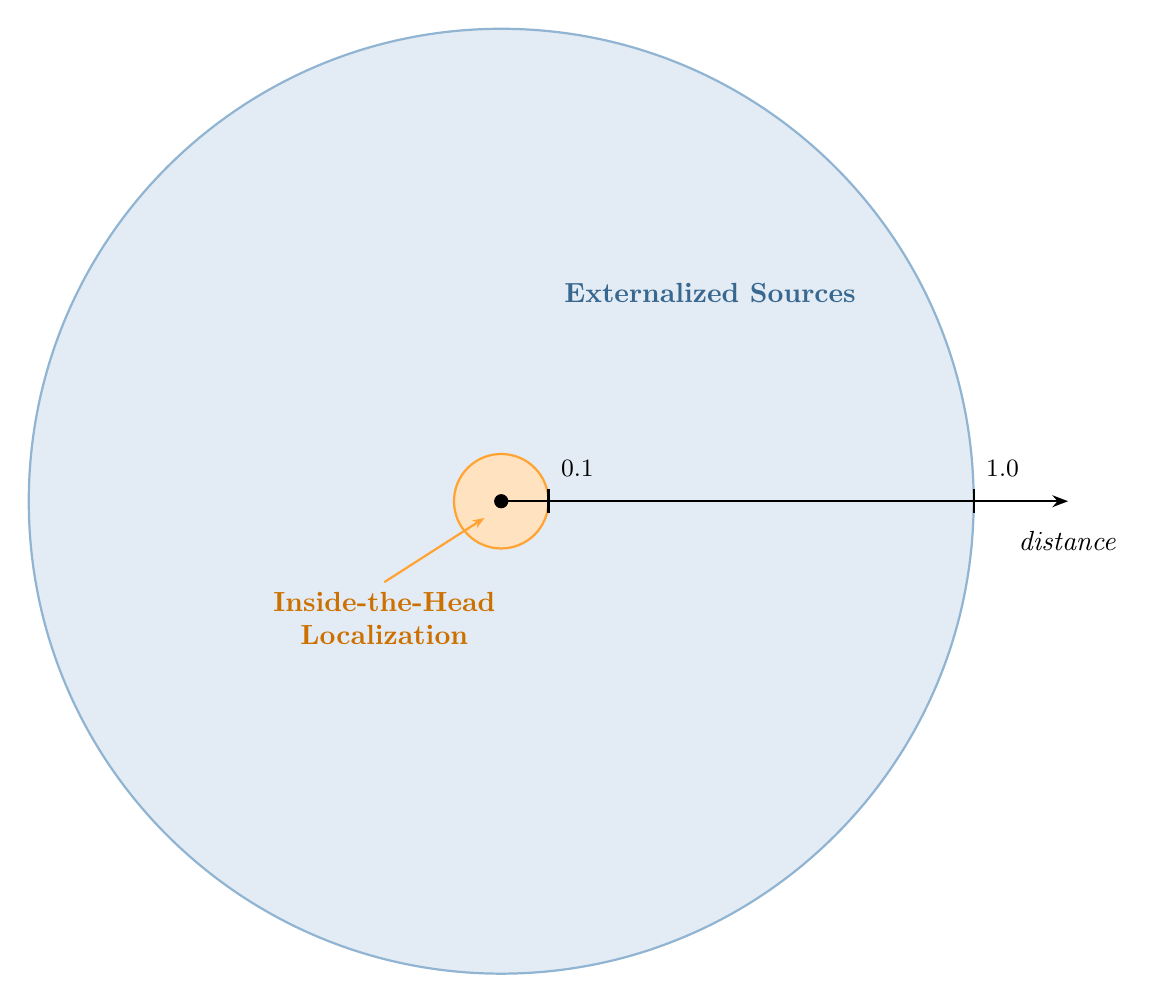
\begin{tikzpicture}[scale=6]

  % Define colors
  \definecolor{innerzone}{RGB}{255,140,0}  % Orange
  \definecolor{outerzone}{RGB}{70,130,180} % Steel Blue

  % outer zone (0.1..1)
  \fill[outerzone!15] (0,0) circle (1);

  % inner in-head-localization zone (0..0.1)
  \fill[innerzone!25] (0,0) circle (0.1);

  % circles outlines
  \draw[thick,outerzone!60] (0,0) circle (1);
  \draw[thick,innerzone!80] (0,0) circle (0.1);

  % listener position at center
  \fill[black] (0,0) circle (0.015);

  % radial axis with enhanced styling
  \draw[-{Stealth[length=2mm]},thick] (0,0) -- (1.2,0);
  \node[below=3pt,font=\normalsize] at (1.2,-0.025) {\textit{distance}};

  % Distance markers with better styling
  \draw[thick] (0.1,0.025) -- (0.1,-0.025);
  \node[above right=1pt,font=\small] at (0.1,0.025) {$0.1$};
  \draw[thick] (1,0.025) -- (1,-0.025);
  \node[above right=1pt,font=\small] at (1,0.025) {$1.0$};

  % Zone labels with better positioning and styling
  \node[align=center,font=\normalsize,outerzone!80!black] at (45:0.625)
    {\textbf{Externalized Sources}};

  % In-Head Localization label with arrow pointing to inner zone
  \node[align=center,font=\normalsize,innerzone!80!black] (inheadlabel) at (225:0.35)
    {\textbf{Inside-the-Head} \\ \textbf{Localization}};
  \draw[-{Stealth[length=1.5mm]},thick,innerzone!80] (inheadlabel.north) -- (225:0.05);

\end{tikzpicture}
\end{document}
